\titre{\tgit}

\begin{quotation}
  \sl Une grande partie de ce TP consiste à lire et comprendre des
  documents sur moodle. Le but n'est pas de le faire le plus
  rapidement possible, mais de comprendre au mieux une architecture
  beaucoup plus complexe que ce que vous avez vu jusque là.
\end{quotation}

\section*{Présentation}

Au cours de ce TP, on va mettre en place les comptes sur différents
sites Web externes qui nous permettront de gérer le code C qui sera
écrit.

\exo{Espace de travail sur Cloud 9}

\question Commencez par ouvrir le mail reçu de \url{support@c9.io} sur
l'adresse mail de l'université, et allez sur la page pour créer un
compte. évitez d'être trop imaginatif sur le nom, prénom, car vous
pourriez être amené à présenter votre travail sur ce compte.

\question Une fois l'inscription terminée, vous recevrez un autre
email avec un lien pour modifier votre mot de passe.

Un \emph{workspace} (espace de travail) correspond à un projet
unique. Cette définition englobe à la fois les fichiers, les
répertoires, mais aussi un ou plusieurs terminaux, ainsi que la
visualisation de l'ensemble. 

\question Créez un \emph{workspace} appelé \texttt{programmation-c} (tout
en minuscules) comme projet \emph{blank} (icône orange Ubuntu
sur la Fig.~\ref{fig:workspace:creation}) et \emph{privé}.

\begin{figure}[htbp]
  \centering
  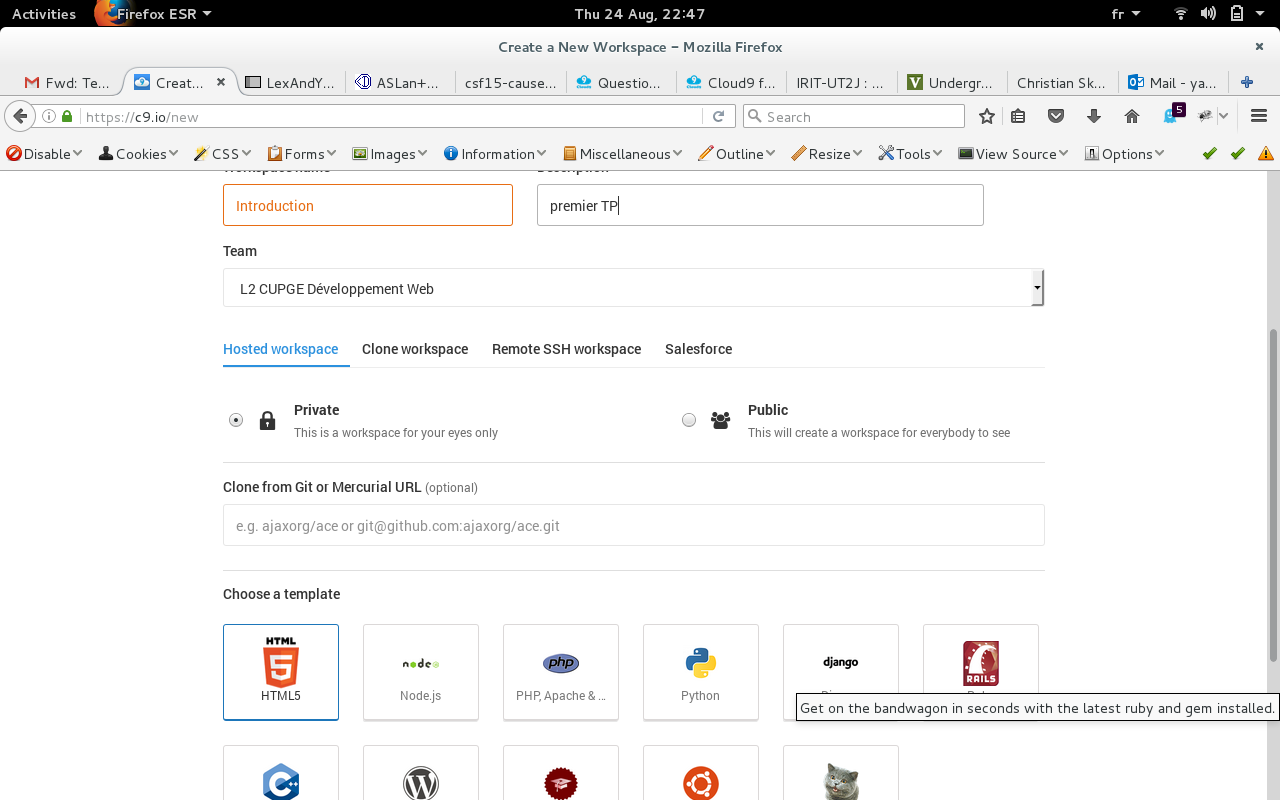
\includegraphics[width=0.9\textwidth]{images/creation_workspace}
  \caption{Fenêtre de création d'un espace de travail.}
  \label{fig:workspace:creation}
\end{figure}

L'environnement de travail ressemble alors à la Fig.~\ref{fig:workspace:initial}.

\begin{figure}[htbp]
  \centering
  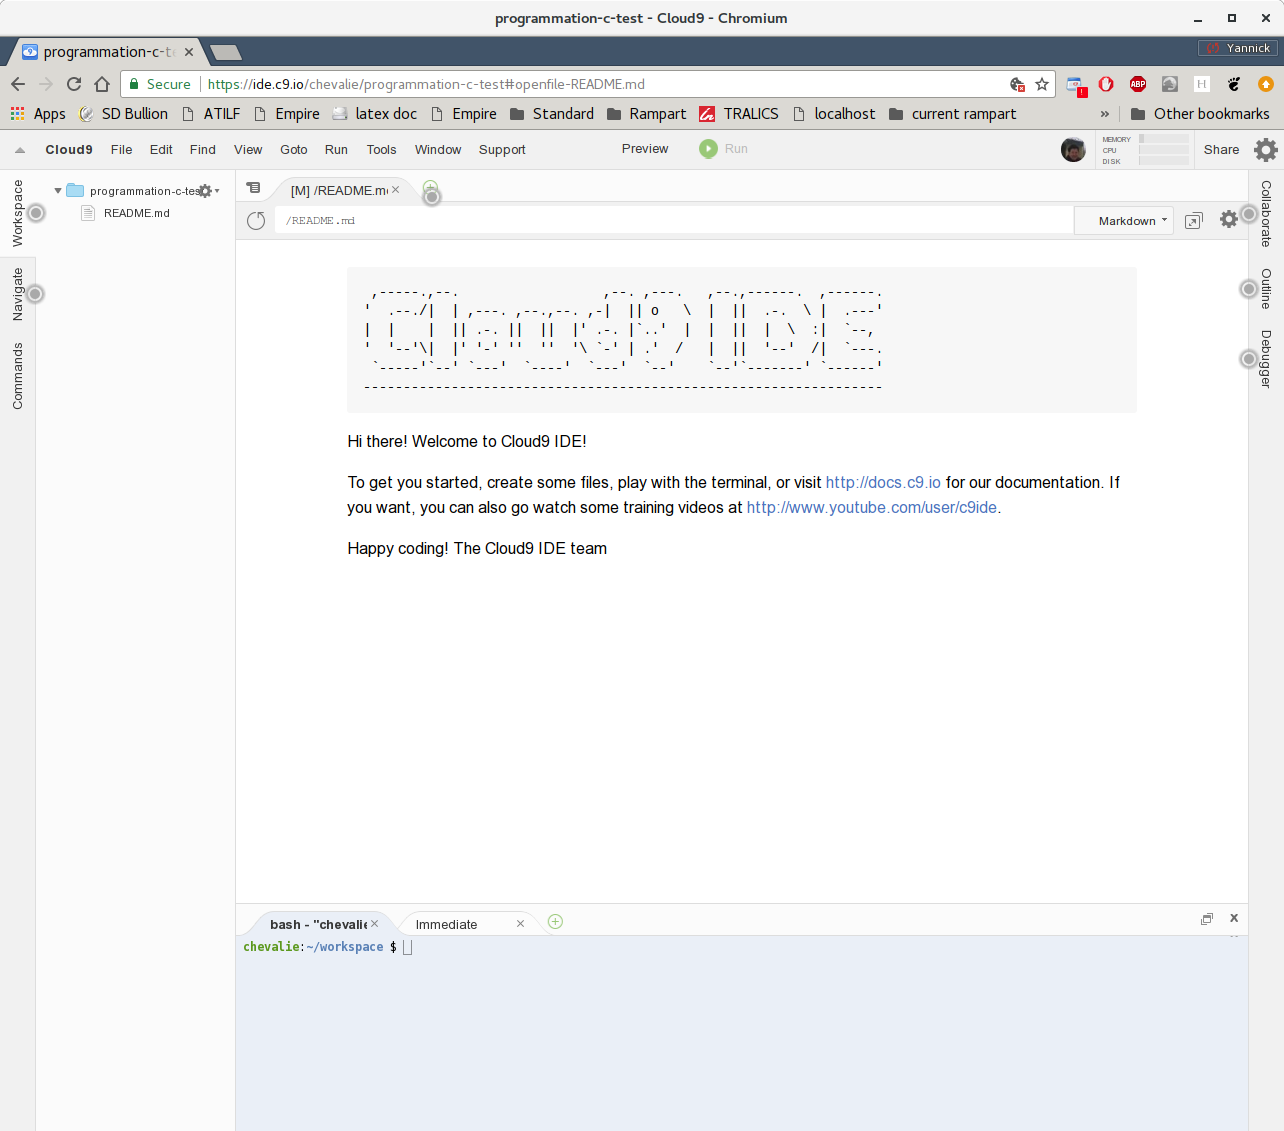
\includegraphics[width=0.9\textwidth]{images/c9_apres_creation.png}
  \caption{Espace de travail intial.}
  \label{fig:workspace:initial}
\end{figure}

\begin{fminipage}{0.9\textwidth}
  Ne fermez pas la fenêtre \url{c9.io}, nous en aurons besoin dans
  l'exercice suivant (il faut ouvrir un nouvel onglet).
\end{fminipage}

\question Par défaut, votre compte sur \url{c9.io} peut être identifié
avec le protocole \texttt{ssh} par une clef publique. Allez dans le répertoire \url{~/.ssh} et affichez la clef privée (qui est stockée dans le fichier \texttt{id\_rsa}) et la clef publique (qui est stockée dans le fichier \texttt{id\_rsa.pub}).

\begin{fminipage}{\textwidth}
  \begin{itemize}
  \item Revenez ensuite dans le répertoire \url{~/workspace/}
  \item \textbf{Tous les TP seront dans ce répertoire}
  \item Le répertoire marqué \url{~/workspace/} a le nom de votre projet dans la
    fenêtre de gauche
  \end{itemize}
\end{fminipage}


\begin{solution}
  \begin{lstlisting}[language=bash]
    cd ~/.ssh
    cat id_rsa
    cat id_rsa.pub
    cd ~/workspace
  \end{lstlisting}
\end{solution}

\exo{Création d'un compte sur BitBucket}

Pour créer un compte sur \url{https://bitbucket.org/}, il faut
utiliser le lien \texttt{sign up}. Il vous sera demandé une adresse
mail à laquelle sera envoyée un e-mail de confirmation d'inscription.


\question Sur l'écran d'accueil, juste après la validation, cliquez
sur l'icône de profil en bas, à gauche pour accéder à votre tableau de
bord (\emph{dashboard}). Puis allez dans votre compte en cliquant sur
l'icône en bas, à gauche, puis \texttt{view profile},
\texttt{settings}, \texttt{Security}, et \texttt{ssh keys}. On va
relier notre espace de travail sur \url{c9.io} en utilisant la clef
publique qu'on a vue à l'exercice précédent.

\question Allez ensuite sur \texttt{overview}, et créez un premier
dépôt (repository) (\texttt{Programmation C}, par exemple) comme dépôt
privé. 
\begin{fminipage}{\textwidth}
  Créez un dépôt vide (sans README.md) pour éviter des conflits plus
  tard.
\end{fminipage}



\exo{Récupérer les énoncés de TP}

Les énoncés de TP sont sur \texttt{\url{http://github.com/}}, un autre
site de gestion de projets utilisant le système de gestion de version git.

\question Téléchargez les énoncés de TP en utilisant la commande suivante:
\begin{lstlisting}[language=bash]
  git clone https://github.com/YannickChevalier/programmation-en-C-CUPGE.git
\end{lstlisting}


\question Allez dans le répertoire qui vient d'êtr copié, et ajoutez
le dépôt que vous avez créé sur bitbucket comme autre dépôt distant:
\begin{lstlisting}[language=bash]
  git remote add bitbucket git@bitbucket.org:NOM/PROJET.git
\end{lstlisting}


\question Mettez à jour le serveur sur BitBucket en fonction de votre
serveur local.  Sur bitbucket, allez dans \texttt{Source} pour
vérifier que tout a bien marché.
\begin{lstlisting}[language=bash]
  git push bitbucket enonces
\end{lstlisting}



\question Éditez le fichier \texttt{README.md} sur C9, sauvegarder (et
``commitez''), et transférer sur BitBucket. Vérifiez que les
transferts marchent correctement.
\begin{lstlisting}[language=bash]
  echo "..."
  git status # découverte des opérations depuis la dernière sauvegarde
  git add . # ajout des fichiers modifiés dans la liste de fichiers à transférer
  git status # vérification de la liste de fichiers à modifier
  git commit -m "Modification du fichier README.md"
  git push bitbucket enonces
\end{lstlisting}
